\documentclass{article}
\usepackage{scicite}
\usepackage{amsmath, amsthm, amsfonts, amssymb}
\usepackage{multirow, microtype, graphicx}
\usepackage{longtable}
\usepackage{lineno}
\bibliographystyle{science}

\renewcommand{\thefigure}{S\arabic{figure}}
\renewcommand{\thetable}{S\arabic{table}}

\setcounter{figure}{0}
\setcounter{table}{0}

\title{Supplementary Text for ``Death and Taxa''}
\author{Peter D Smits}

\begin{document}
\maketitle
\linenumbers
\modulolinenumbers[2]

\section{Materials and Methods}

\subsection{Species occurrence and covariate information}
Fossil occurrence information was downloaded from the Paleobiology Database (PBDB; http://paleodb.org/). Occurrence, taxonomic, stratigraphic, and biological information was downloaded for all North American mammals. This data set was filtered so that only occurrences identified to the species-level, excluding all ``sp.''-s. All aquatic and volant taxa were also excluded. Additionally, all occurrences without latitude and longitude information were excluded from the sample.

Species dietary and locomotor category assignments were done using the assignments in the PBDB, which were then reassigned into coarser categories (Table \ref{tab:trait_cats}). This was done to improve interpretability, increase sample size per category, and make results comparable to previous studies \cite{Jernvall2004,Price2012}.

All individual fossil occurrences were assigned to 2 My bins ranging through the entire Cenozoic. Taxon duration was measured as the number of bins from the first occurrence to the last occurrence, inclusive. This bin size was chosen because it approximately reflects the resolution of the North American Cenozoic mammal fossil record \cite{Alroy2009,Alroy2000g,Marcot2014}. The youngest cohort, 0-2 My, was excluded from analysis.


\subsubsection{Body size estimates and estimation}
Species body size estimates were sourced from a large selection of primary literature and data base compilations.

Databases used include the PBDB, PanTHERIA \cite{Jones2009c}, and the Neogene Old World Mammal database (NOW; http://www.helsinki.fi/science/now/). Major sources of additional compiled body size estimates include \cite{Brook2004a,Freudenthal2013,McKenna2011,Raia2012f,Smith2004c,Tomiya2013}. These were then supplemented with an additional literature search to try and fill in the remaining gaps. In many cases, species body mass was estimated using various published regression equations based on tooth or skull measurements (Tab. \ref{tab:mass_est}). See Supplementary Tables XXX for a complete list of individual measures and sources.

\subsubsection{Biogeographic network}
Species geographic extent was characterized using a network-theoretic approach that has previously been applied to paleontological data \cite{Sidor2013,Vilhena2013}. This approach relies on defining a biogeographic bipartite network of taxa and localities. In this study, taxa were defined as species and localities were grid cells from a regular lattice on a global equal-area cylinder map projection. The regular lattice was defined as a 70 x 34 global grid where each cell corresponds to approximately 25 km\(^{2}\). This network is considered bipartite because taxa are connected to localities based on their occurrence but taxa are not connected to taxa nor are localities connected to localities.

A biogeographic network was constructed for each of the 2 My bins used in this study. Emergent bioprovinces were then identified using the map equation \cite{Rosvall2008,Rosvall2009a} as has been done before \cite{Sidor2013,Vilhena2013b,Vilhena2013}. These bioprovinces correspond to taxa and localities that are more interconnected with each other than with other nodes.

The map projection and regular lattice were made using shape files from http://www.naturalearthdata.com/ and the \texttt{raster} package for R \cite{raster}. The map equation and other network related analysis was done using the \texttt{igraph} package for R \cite{csardi2006igraph}.


\subsubsection{Supertree}

As there is no single, combined formal phylogenetic hypothesis of all Cenozoic fossils mammals from North America, it was necessary to construct a semi-formal supertree. This was done by combining taxonomic information for all the observed species and a few published phylogenies.

The initial taxonomic classification of the observed species was based on the associated taxonomic information from the PBDB. This information was then updated using the Encyclopedia of Life (http://eol.org/) which collects and collates taxonomic information in a single database. This was done programatically using the \texttt{taxize} package for R \cite{2013taxize}. Finally, this taxonomic information was further updated using a published taxonomy of fossil mammals \cite{Janis2008,Janis1998}. 

This taxonomy serves as an initial phylogenetic hypothesis which was then combined with a selection of species-level phylogenies \cite{Bininda-Emonds2007,Raia2012f} in order to better constrain a minimum estimate of the actual phylogenetic relationships of the species. The supertree was inferred via matrix representation parsimony implemented in the \texttt{phytools} package for R \cite{revell2012phytools}. While four most parsimonious trees were found, I selected a single of these for use in analysis.

Polytomies were resolved in order of species first appearance in order to minize stratigraphic gaps. The resulting tree was then time scaled using the \texttt{paleotree} package via the ``minimum branch length'' approach with a minimum length of 0.1 My \cite{Bapst2012a}. The minimum length is necessary to avoid zero-length branches which cause the phylogenetic covariance matrix to not be positive definite, which is important for computation (see below). While other time scaling approaches are possible \cite{Bapst2013a,Hedman2010} this method was chosen for its simplicity and not requiring additional information about diversification rates which are the interest of this study. 


\subsection{Survival model}
Presented here is the model development process used to formulate the two survival models used in this study. 

First, define \(y\) as a vector of length \(n\) where the \(i\)th element is the duration of species \(i\) where \(i = 1,\cdots,n\).

The simplest survival model where durations are assumed to follow an exponential distribution with a single ``rate'' or inverse-scale parameter \(\lambda\) \cite{Klein2003}. This is written out as
\begin{align}
  p(y | \lambda) &= \lambda \exp(-\lambda y) \nonumber \\
  y &\sim \mathrm{Exp}(\lambda).
  \label{eq:exp}
\end{align}
The exponential distribution corresponds to situations where extinction risk is independent of age. To understand this, we need to define two functions: the survival function \(S(t)\) and the hazard function \(h(t)\). 

\(S(t)\) corresponds to the probability that a species having existed for \(t\) My will not have gone extinct while \(h(t)\) corresponds to the instantaneous extinction rate for some taxon age \(t\) \cite{Klein2003}. For an exponential model, \(S(t)\) is defined
\begin{equation}
  S(t) = \exp(-\lambda t)
  \label{eq:exp_surv}
\end{equation}
and \(h(t)\) is defined
\begin{equation}
  h(t) = \lambda
  \label{eq:exp_haz}
\end{equation}
The choice of the exponential distribution corresponds directly to the Law of Constant Extinction \cite{VanValen1973} as the right side of Eq. \ref{eq:exp_haz} does not depend on species age \(t\). 

The current sampling statement (Eq. \ref{eq:exp}) assumes that all species share the same rate parameter with no variation. To allow for variation in \(\lambda\) associated with relevant covariate information like species body size, \(\lambda\) is reparameterized as \(\lambda_{i} = \exp(\sum \beta^{T}\mathbf{X}_{i})\) with \(i\) indexing a given observation and its covariates, \(\beta\) is a vector of regression coefficients, and \(\mathbf{X}\) is a matrix of covariates. This is a standard regression formulation, where one column of \(\mathbf{X}\) is all 1-s and its corresponding \(\beta\) coefficient is the intercept. This approach is essentially a generalized linear model (GLM) approach where instead of normally distributed errors there are exponentially distributed errors \cite{Klein2003}.

To relax the assumption of age-independent extinction of the Law of Constant Extinction we substitute the Weibull distribution for the exponential \cite{Klein2003}. The Weibull distribution has a shape parameter \(\alpha\) and scale parameter \(\sigma\). Conceptually, \(\sigma\) is the inverse of \(\lambda\). \(\alpha\) modifies the impact of taxon age on extinction risk. When \(\alpha > 1\) then \(h(t)\) is a monotonically increasing function, but when \(\alpha < 1\) then \(h(t)\) is a monotonically decreasing function. When \(\alpha = 1\) then the Weibull distribution is equivalent to the exponential.

The Weibull distribution and sampling statement wre defined
\begin{align}
  p(y | \alpha, \sigma) &= \frac{\alpha}{\sigma} \left(\frac{y}{\sigma}\right)^{\alpha - 1} \exp\left(-\left(\frac{y}{\sigma}\right)^{\alpha}\right) \nonumber \\
  y &\sim \mathrm{Weibull}(\alpha, \sigma).
  \label{eq:weibull}
\end{align}
The corresponding \(S(t)\) and \(h(t)\) functions are defined
\begin{align}
  S(t) &= \exp\left(-\left(\frac{t}{\sigma}\right)^{\alpha}\right) \label{eq:wei_surv} \\
  h(t) &= \frac{\alpha}{\sigma}\left(\frac{t}{\sigma}\right)^{\alpha - 1} \label{eq:wei_haz}.
\end{align}

To allow for \(\sigma\) to vary with a given observation's covariate information it is reparameterized in a similar fashion to \(\lambda\) with a few key differences. Because \(\sigma = 1/\lambda\) in order to preserve the interpretation of \(\beta\), while taking \(\alpha\) into account, \(\sigma\) is reparameterized as
\begin{equation}
  \sigma_{i} = \exp\left(\frac{-(\beta_{0}}{\alpha}\right)
  \label{eq:reg}
\end{equation}
where \(\beta_{0}\) is the intercept term.

The model described here was the final model at the end of a continuous model development framework where the sampling and prior distributions were iteratively modified to best reflect theory, knowledge of the data, the inclusion of important covariates, and the fit to the data. This follows the approach described in \cite{Gelman2007} and \cite{Gelman2013d}.
A survival model was fit in a Bayesian context where species duration were assumed to be drawn from a Wiebull distribution (Eq. \ref{eq:weibull}) with shape \(\alpha\) and scale \(\sigma\) parameters. \(\alpha\) was assumed constant, which is standard practice in survival analysis \cite{Klein2003}. \(\alpha\) was given a weakly informative half-Cauchy (C\(^{+}\)) prior. \(\sigma\) was reparameterized as an exponentiated regression model (Eq. \ref{eq:reg}). This was further expanded (Eq. \ref{eq:wei_reg_ext}) to allow for two hierarchical factors as discussed below. This is written
\begin{equation}
  \sigma_{i} = \exp\left(\frac{-(h_{i} + \eta_{j[i]} + \sum \beta^{T} \mathbf{X}_{i})}{\alpha}\right)
  \label{eq:wei_reg_ext}
\end{equation}
where equivalent statement for the exponential distribution is defined
\begin{equation}
  \lambda_{i} = \exp\left(h_{i} + \eta_{j[i]} + \sum \beta^{T} \mathbf{X}_{i})\right).
  \label{eq:exp_reg_ext}
\end{equation}

\(\mathbf{X}\) is an \(n \times K\) matrix of species-level covariates. Three of the covariates of interest are the logit of mean relative occupancy, logarithm of body size (g), and interaction between these two terms. The discrete covariate index variables of dietary and locomotor category were transformed into \(n \times (k - 1)\) matrices where each column is an indicator variable (0/1) for that species's category, \(k\) being the number of categories of the index variable (3 and 4, respectively). Only \(k - 1\) indicator variables are necessary as the intercept takes on the remaining value. Finally, a vector of 1-s was included in the matrix \(\mathbf{X}\) whose corresponding \(\beta\) coefficient is the intercept, making \(K\) equal nine.

\(\beta\) is the vector of regression coefficients. The intercept term was given a weak normal prior, \(\beta_{0} \sim \mathcal{N}(0, 10)\) while all of these other coefficients were slightly more informative priors, e.g. \(\beta_{mass} \sim \mathcal{N}(0, 5)\). These priors were chosen because it is expected that the effect size of each variable on duration will be small, as is generally the case with binary covariates \cite{Gelman2007}. %In all cases, posterior inference was not effected by changes to this choice of prior. Do I have proof?

Regression coefficients are not directly comparable without first standardizing the input variables to have equal standard deviations. This is accomplished by subtracting the mean of the covariate from all values and then dividing by the standard deviation, resulting in a variable with mean of zero and a standard deviation of one. This linear transform greatly improves the interpretability of the coefficients as expected change in mean duration given a difference of one standard deviation in the covariate \cite{Schielzeth2010}. Additionally, this makes the intercept directly interpretable as the estimate of mean (transformed) \(\sigma\) (Eq. \ref{eq:reg}). However, because the expected standard deviation for a binary variable is 0.5, in order to make comparisons between the binary and continuous variables, the continuous inputs must instead be divided by twice their standard deviation \cite{Gelman2008}. 

\subsubsection{Hierarchical effects}

The two hierarchical effects of interest in this study are origination cohort and shared evolutionary history, or phylogeny. Hierarchical modeling can be considered an intermediate between complete and no pooling of groups \cite{Gelman2007}, where complete pooling is when the differences between groups are ignored and no pooling is where different groups are analyzed separately. By allowing for partial pooling, we are modeling the appropriate compromise between these two extremes, allowing for better and potentially more informative overall inference. This is done by having all of the groups share the same Normal prior with mean 0 and a scale parameter estimated from the data, which then acts as an indicator of the amount of pooling. A scale of 0 and \(\infty\) indicate complete and no pooling, respectively. The choice of mean 0 allows for the individual group estimates to be interpreted as deviations from the intercept. Hierarchical modeling is analogous to mixed-effects modeling \cite{Gelman2007}.

Origination cohort is defined as the group of species which all originated during the same 2 My temporal bin. Because the most recent temporal bin, 0-2 Mya, was excluded, there are 32 different cohorts. The effect of origination cohort \(j\) was modeled with each group being a sample from a common cohort effect, \(\eta\), which was considered Normally distributed with mean 0, and standard deviation \(\sigma_{c}\). The value of \(\sigma_{c}\) was then estimated from the data itself, corresponding to the amount of pooling in the individual estimates of \(\eta_{j}\). This approach is a conceptual and statistical unification between dynamic and cohort survival analysis in paleontology \cite{Foote1988,Raup1978,Raup1975,VanValen1979,Baumiller1993}, with \(\sigma_{c}\) acting as a measure of compromise between these two end members.

\begin{align*}
  \eta_{j} &\sim \mathcal{N}(0, \sigma_{c}) \\
  \sigma_{c} &\sim \mathrm{C}^{+}(0, 2.5)
\end{align*}

The choice of the half-Cauchy prior on \(\sigma_{c}\) follows \cite{Gelman2006a}.

The impact of shared evolutionary history, or phylogeny, was modeling as an individual effect where each observation, \(i\), is modeled as a multivariate normal, \(h\), where the covariance matrix \(\Sigma\) is known up to a constant, \(\sigma_{p}^{2}\) \cite{Lynch1991,Housworth2004}. This is written

\begin{align*}
  h &\sim \mathrm{Multivariate\ }\mathcal{N}(0, \mathbf{\Sigma}) \\
  \mathbf{\Sigma} &= \sigma_{p}^{2} \mathbf{V}_{phy} \\
  \sigma_{p} &\sim \mathrm{C}^{+}(0, 2.5).
\end{align*}

\(\mathbf{V}_{phy}\) is the phylogenetic covariance matrix defined as an \(n \times n\) matrix where the diagonal elements are the distance from root to tip, in branch length, for each observation and the off-diagonal elements are the amount of shared history, measured in branch length, between observations \(i\) and \(j\). \(\sigma_{p}\) was given a weakly informative half-Cauchy hyperprior. 


\subsubsection{Censored observations} \label{sec:censor}

An important part of survival analysis is the inclusion of censored observations where the failure time has not been observed \cite{Ibrahim2001,Klein2003}. The most common censored observation is right censored, where the point of extinction had not yet been observed in the period of study, such as taxa that are still extant. Left censored observations, on the other hand, correspond to observations that went extinct any time between 0 and some known point. In order to account for the minimum resolution of the fossil record encountered here, taxa that occurred in only a single time bin were left censored.

Censored data are modeled using the survival function of the distribution, \(S(t)\), defined earlier for the Weibull distribution (Eq. \ref{eq:wei_surv}) with \(\sigma\) defined as above (Eq. \ref{eq:wei_reg_ext}). \(S(t)\) is the probability that an observation will survive longer than a given time \(t\). The likelihood of uncensored observations is evaluated as normal using Equation \ref{eq:weibull} while right censored observations are evaluated at \(S(t)\) and left censored observations are evaluated at \(1 - S(t)\). Note, \(1 - S(t)\) is equivalent to the cumulative distribution function and \(S(t)\) is equivalent to the complementary cumulative distribution function \cite{Gelman2013d}.

The full likelihood for both uncensored and both right and left censored observations is written
\begin{equation*}
  L \propto \prod_{i \in C} \mathrm{Weibull}(y_{i} | \alpha, \sigma) \prod_{j \in R} S(y_j | \alpha, \sigma) \prod_{k \in L} \left(1 - S(y_{k} | \alpha, \sigma)\right),
\end{equation*}
where \(C\) is the set of uncensored observations, \(R\) is the set of right censored observations, and \(L\) is the set of left censored observations.


\subsubsection{Estimation}
Parameter posteriors were approximated using a Markov-chain Monte Carlo (MCMC) routine implemented in the Stan programming language \cite{2014stan}. Stan implements a Hamiltonian Monte Carlo using a No-U-Turn sampler \cite{Hoffman-Gelman:2011}. Posterior approximation was done using four parallel MCMC chains run for 30000 steps, thinned to every thirtieth sample, split evenly between warm-up and sampling. Convergence was evaluated using the scale reduction factor, \(\hat{R}\). Values of \(\hat{R}\) close to 1, or less than or equal to 1.1, indicate approximate convergence. Convergence means that the chains are approximately stationary and the samples are well mixed \cite{Gelman2013d}.

In order to speed up the posterior approximation, a custom multivariate normal sampler was used to estimate the unknown constant term in the covariance matrix. This is necessary because inverting and solving the complete covariance matrix on every iteration is a memory intense procedure. The custom sampler limits the necessary number of operations and matrix inversions per iteration.


\subsection{Posterior predictive checks}

The most basic assessment of model fit is that simulated data generated using the fitted model should be similar to the observed. This is the idea behind posterior predictive checks. Using the covariates from each of the observed durations, and randomly drawn parameter estimates from their marginal posteriors, a simulated data set \(y^{rep}\) was generated. This process was repeated 1000 times and the distribution of \(y^{rep}\) was compared with the observed \cite{Gelman2013d}.

An example posterior predictive check used in this study is a graphical comparison between the Kaplan-Meier (K-M) survival curve estimated from the observed data and the K-M survival curves estimated from 1000 simulation sets. K-M survival curves are non-parametric estimates of \(S(t)\) \cite{Klein2003}. Other posterior predictive checks used here include comparison of the mean and quantiles of the observed durations to the distributions of the same quantities from the simulations, and inspection of the deviance residuals, defined below.

In standard linear regression, residuals are defined as \(r_{i} = y_{i} - y_{i}^{est}\). For the model used here, this definition is inadequate. The equivalent values for survival analysis are deviance residuals. To define how deviance residuals are calculated, we first define the cumulative hazard function \cite{Klein2003}. Given \(S(t)\) (Eq. \ref{eq:wei_surv}), we define the cumulative hazard function as 
\begin{equation*}
  \Lambda(t) = -log\left(S\left(t\right)\right).
\end{equation*}

Next, we define martingale residuals \(m\) as
\begin{equation*}
  m_{i} = I_{i} - \Lambda(t_i).
\end{equation*}
\(I\) is the inclusion vector of length \(n\), where \(I_{i} = 1\) means the observation is completely observed and \(I_{i} = 0\) means the observation is censored. Martingale residuals have a mean of 0, range between 1 and \(-\infty\), and can be viewed as the difference between the observed number of deaths between 0 and \(t_{i}\) and the expected number of deaths based on the model. However, martingale residuals are asymmetrically distributed, and can not be interpreted in the same manner as standard residuals. 

The solution to this is to use the deviance residuals, \(D\). This is defined as a function of martingale residuals and takes the form
\begin{equation*}
  D_{i} = \text{sign}(m_{i}) \sqrt{-2[m_{i} + I_{i}log(I_{i} - m_{i})]}.
\end{equation*}
Deviance residuals have a mean of 0 and a standard deviation of 1 by definition.


\subsection{Variance partitioning}
There are three different variance components in this model: sample \(\sigma_{y}^{2}\), cohort \(\sigma_{c}^{2}\), and phylogenetic \(\sigma_{p}^{2}\). The sample variance, \(\sigma_{y}^{2}\), is similar to the residual variance from a normal linear regression. Partitioning the variance between these sources allows the relative amount of unexplained variance of the sample to be compared. However, the Weibull based model used here (Eq. \ref{eq:weibull}) does not include an estimate of the sample variance, \(\sigma_{y}^{2}\). Partitioning the variance between these three components was approximated via a simulation approach modified from \cite{Goldstein2002}.

The procedure is as follows:
\begin{enumerate}
  \item Simulate \(w\) (50,000) values of \(\eta\); \(\eta \sim \mathcal{N}(0, \sigma_{c})\).
  \item For a given value of \(\beta^{T} \mathbf{X}\), calculate \(\sigma^{c*}\) (Eq. \ref{eq:reg}) for all \(w\) simulations, holding \(h\) constant at 0.
  \item Calculate \(\upsilon_{c}\), the Weibull variance (Eq. \ref{eq:wei_var}) of each element of \(\sigma^{c*}\) with \(\alpha\) drawn from the posterior estimate.
  \item Simulate \(w\) values of \(h\); \(h \sim \mathcal{N}(0, \sigma_{p})\). 
  \item For a given value of \(\beta^{T} \mathbf{X}\), calculate \(\sigma^{p*}\) (Eq. \ref{eq:reg}) for all \(w\) simulations, holding \(\eta\) constant at 0.
  \item Calculate \(\upsilon_{p}\), the Weibull variance (Eq. \ref{eq:wei_var}) of each element of \(\sigma^{p*}\) with \(\alpha\) drawn from the posterior estimate.
  \item \(\sigma_{y*}^{2} = \frac{1}{2} \left(\left(\frac{1}{w} \sum_{i}^{w} \upsilon_{pi}\right) + \left(\frac{1}{w} \sum_{j}^{w} \upsilon_{cj}\right)\right)\).
  \item \(\sigma_{c*}^{2} = var(\upsilon_{c})\) and \(\sigma_{p*}^{2} = var(\upsilon_{p})\).
\end{enumerate}

The simulated values of \(h\) were drawn from a univariate normal distribution because each simulated value is in isolation, so there is no concern of phylogenetic autocorrelation. The chosen value for \(\beta^{T} \mathbf{X}\) was a draw from the posterior estimate of the intercept. Because input variables were standardized prior to model fitting, the intercept corresponds to the estimated effect on survival of the sample mean.

Weibull variance is calculated as
\begin{equation}
  var(x) = \sigma^{2}\left(\Gamma\left(1 + \frac{2}{\alpha}\right) - \left(\Gamma\left(1 + \frac{1}{\alpha}\right)\right)^{2}\right),
  \label{eq:wei_var}
\end{equation}
where \(\Gamma\) is the gamma function. 

The variance partitioning coefficients are then calculated, for example, as \(VPC_{phylo} = \frac{\sigma_{p*}^{2}}{\sigma_{y*}^{2} + \sigma_{c*}^{2} + \sigma_{p*}^{2}}\) and similarly for the other components.

I used variance partitioning coefficients (VPC) to estimate the relative importance of the different variance components \cite{Gelman2007}. Phylogenetic heritability, \(h_{p}^{2}\) \cite{Lynch1991,Housworth2004}, is identical to the VPC of the phylogenetic effect. Additionally, because phylogenetic effect was estimated using a principally taxonomy based tree the estimates derived here can be considered minimum estimates of the phylogenetic effect.


\section{Results of posterior predictive checks}
With all marginal posterior estimates having converged (\(\hat{R} < 1.1\)) it is possible to examine the quality of model fit (Table \ref{tab:post_sum}). If the model is an adequate descriptor of the observed data, then relatively confident inference can be made \cite{Gelman2013d}.

Visual examination of the deviance residuals from twelve different sets of posterior predictive simulations indicates few systematic problems (Fig. \ref{fig:ppc_res}). The only concern is that the residuals are slightly skewed however this bias appears very small. This is confirmed by comparing the K-M estimate of the empirical survival function to 100 estimated survival functions from posterior simulations (Fig. MAIN TEXT).

Comparisons of the observed 25th, 50th, and 75th quantiles, and mean durations to the results from the posterior predictive simulations indicate adequate model fit (Fig. \ref{fig:ppc_quant}). Because all the different posterior predictive checks seem to agree, the inferred model appears adequate at capturing the observed variation.


\clearpage

\section{Supplementary figures}

\begin{figure}[ht]
  \centering
  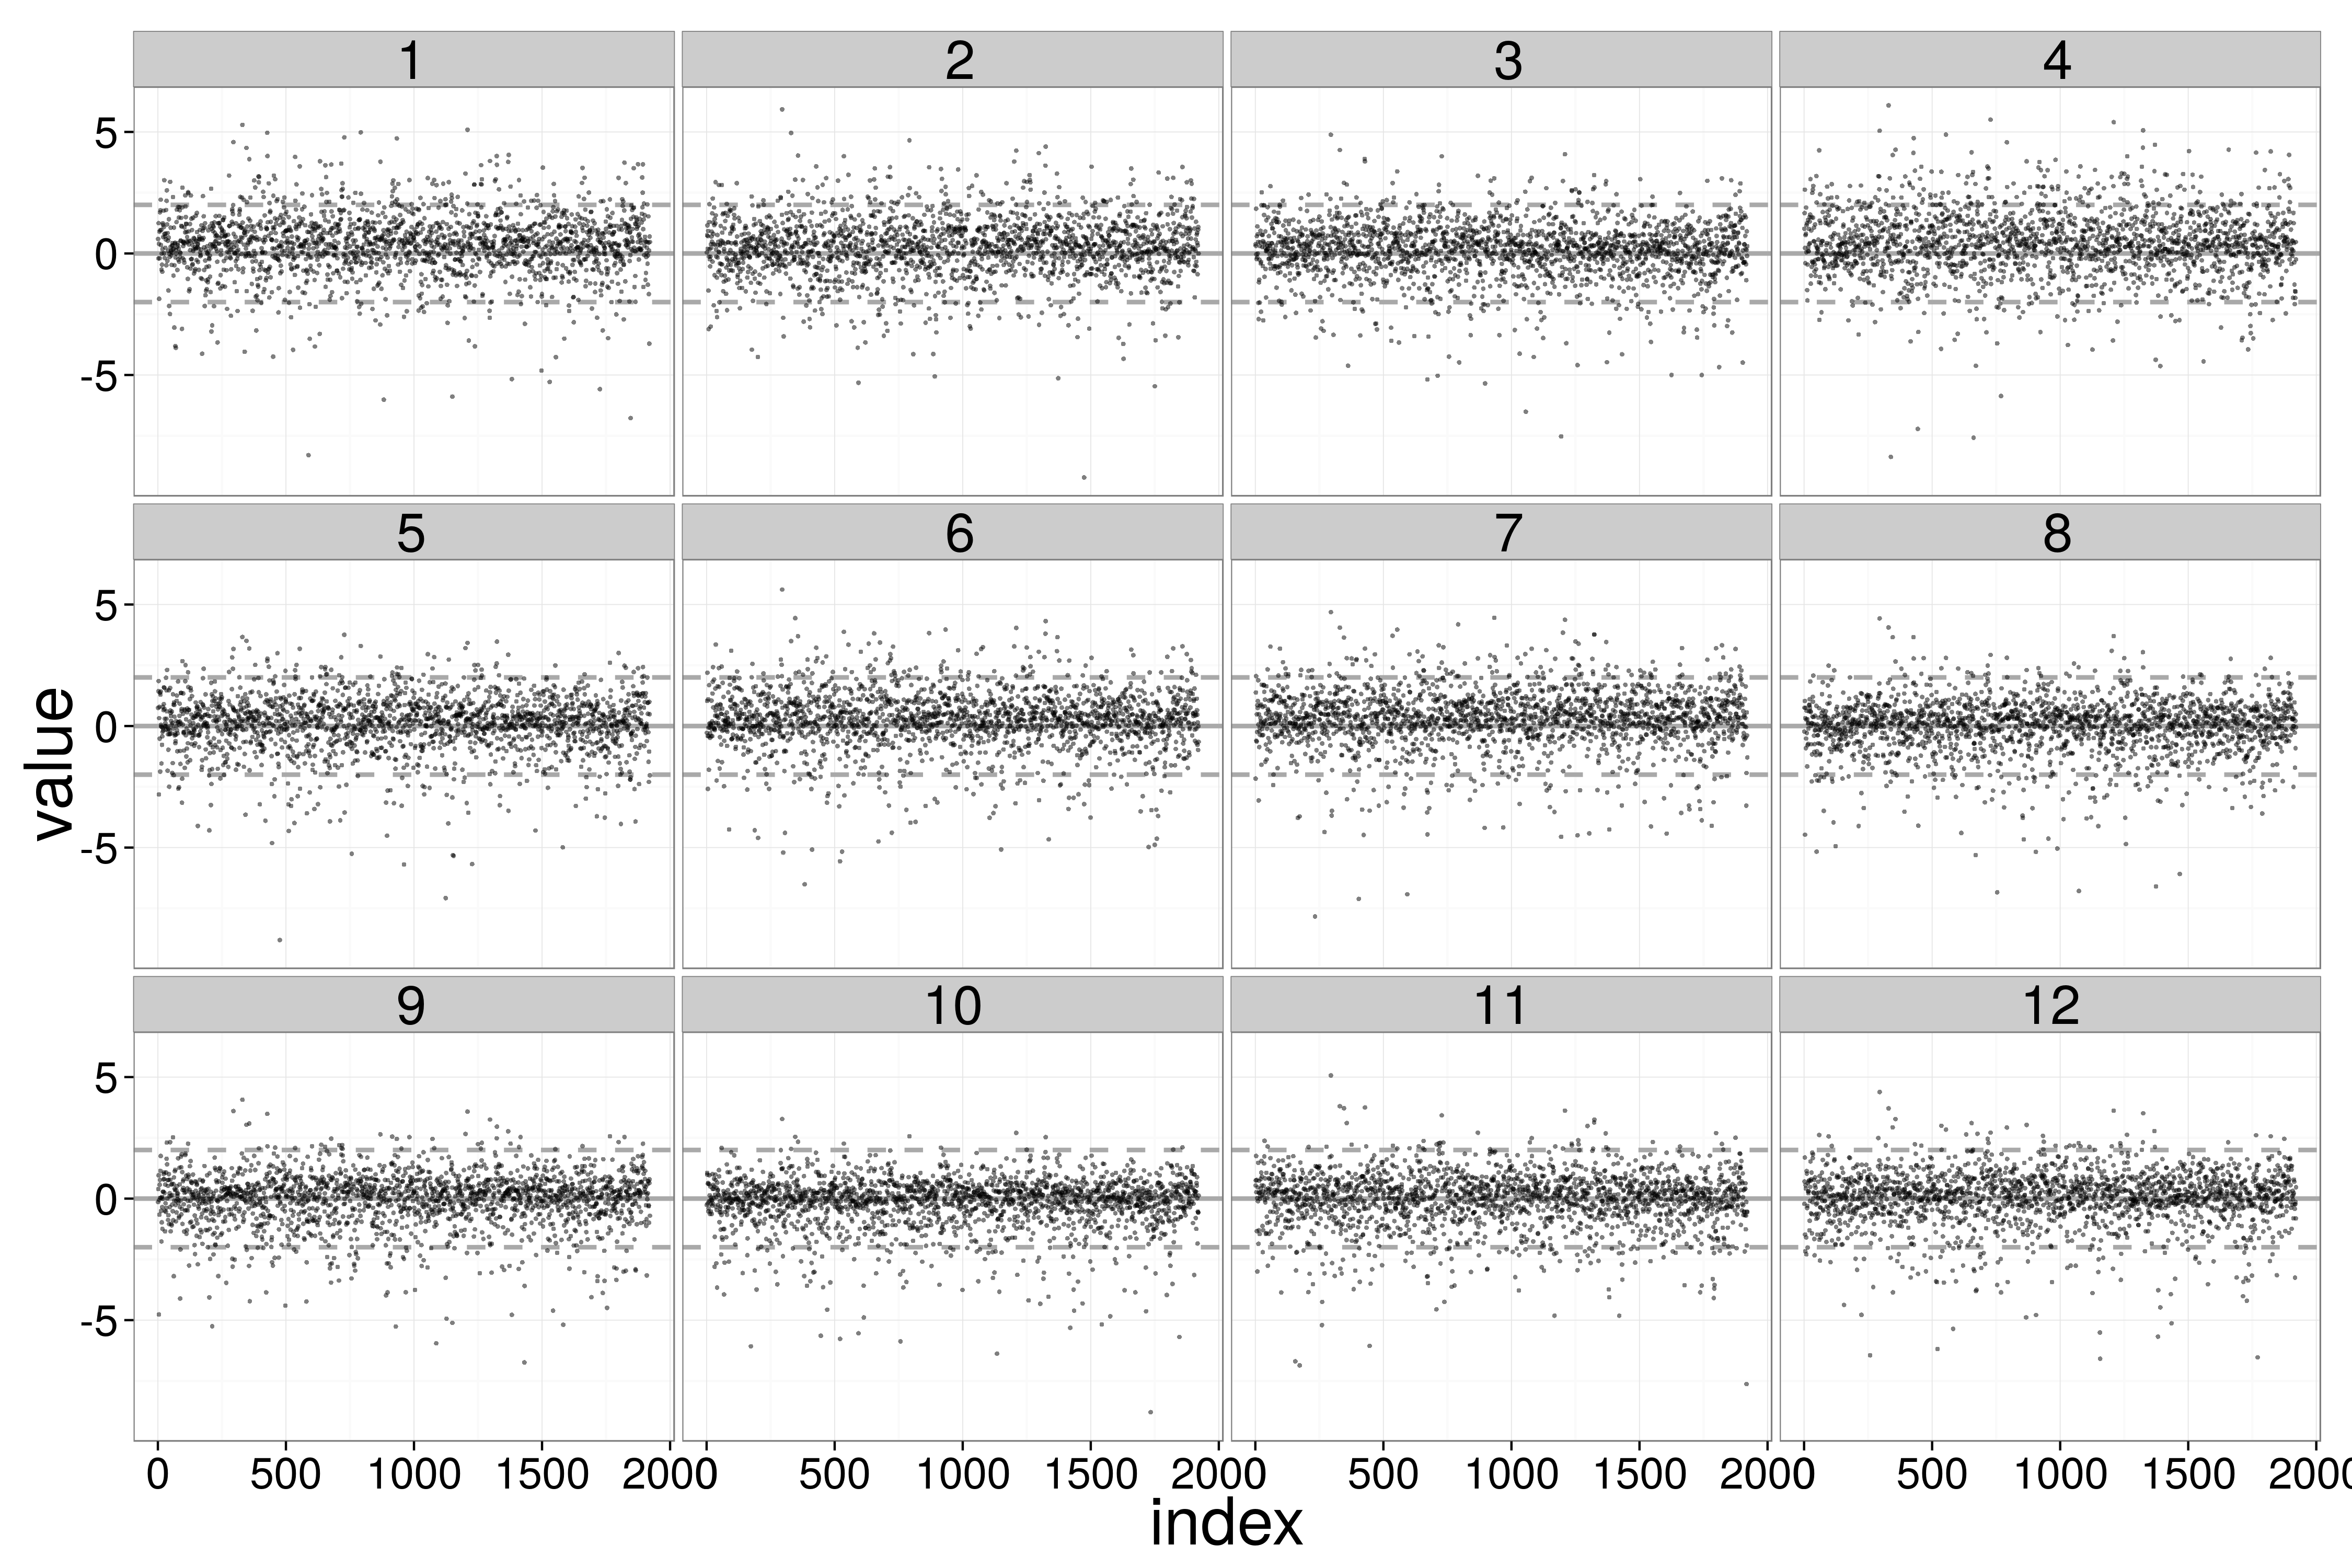
\includegraphics[height = 0.5\textheight, width = \textwidth, keepaspectratio = true]{figure/residual_plot}
  \caption{Deviance residuals from the fitted survival model. Each graph depicts the residuals from single draws from the posterior distributions of all estimated parameters. Positive values indicate an underestimate of the observed duration, while negative values indicate an overestimate of the observed duration. Twelve different examples are provided here to indicate the lack of individual observation based biases.}
  \label{fig:ppc_res}
\end{figure}

\begin{figure}[ht]
  \centering
  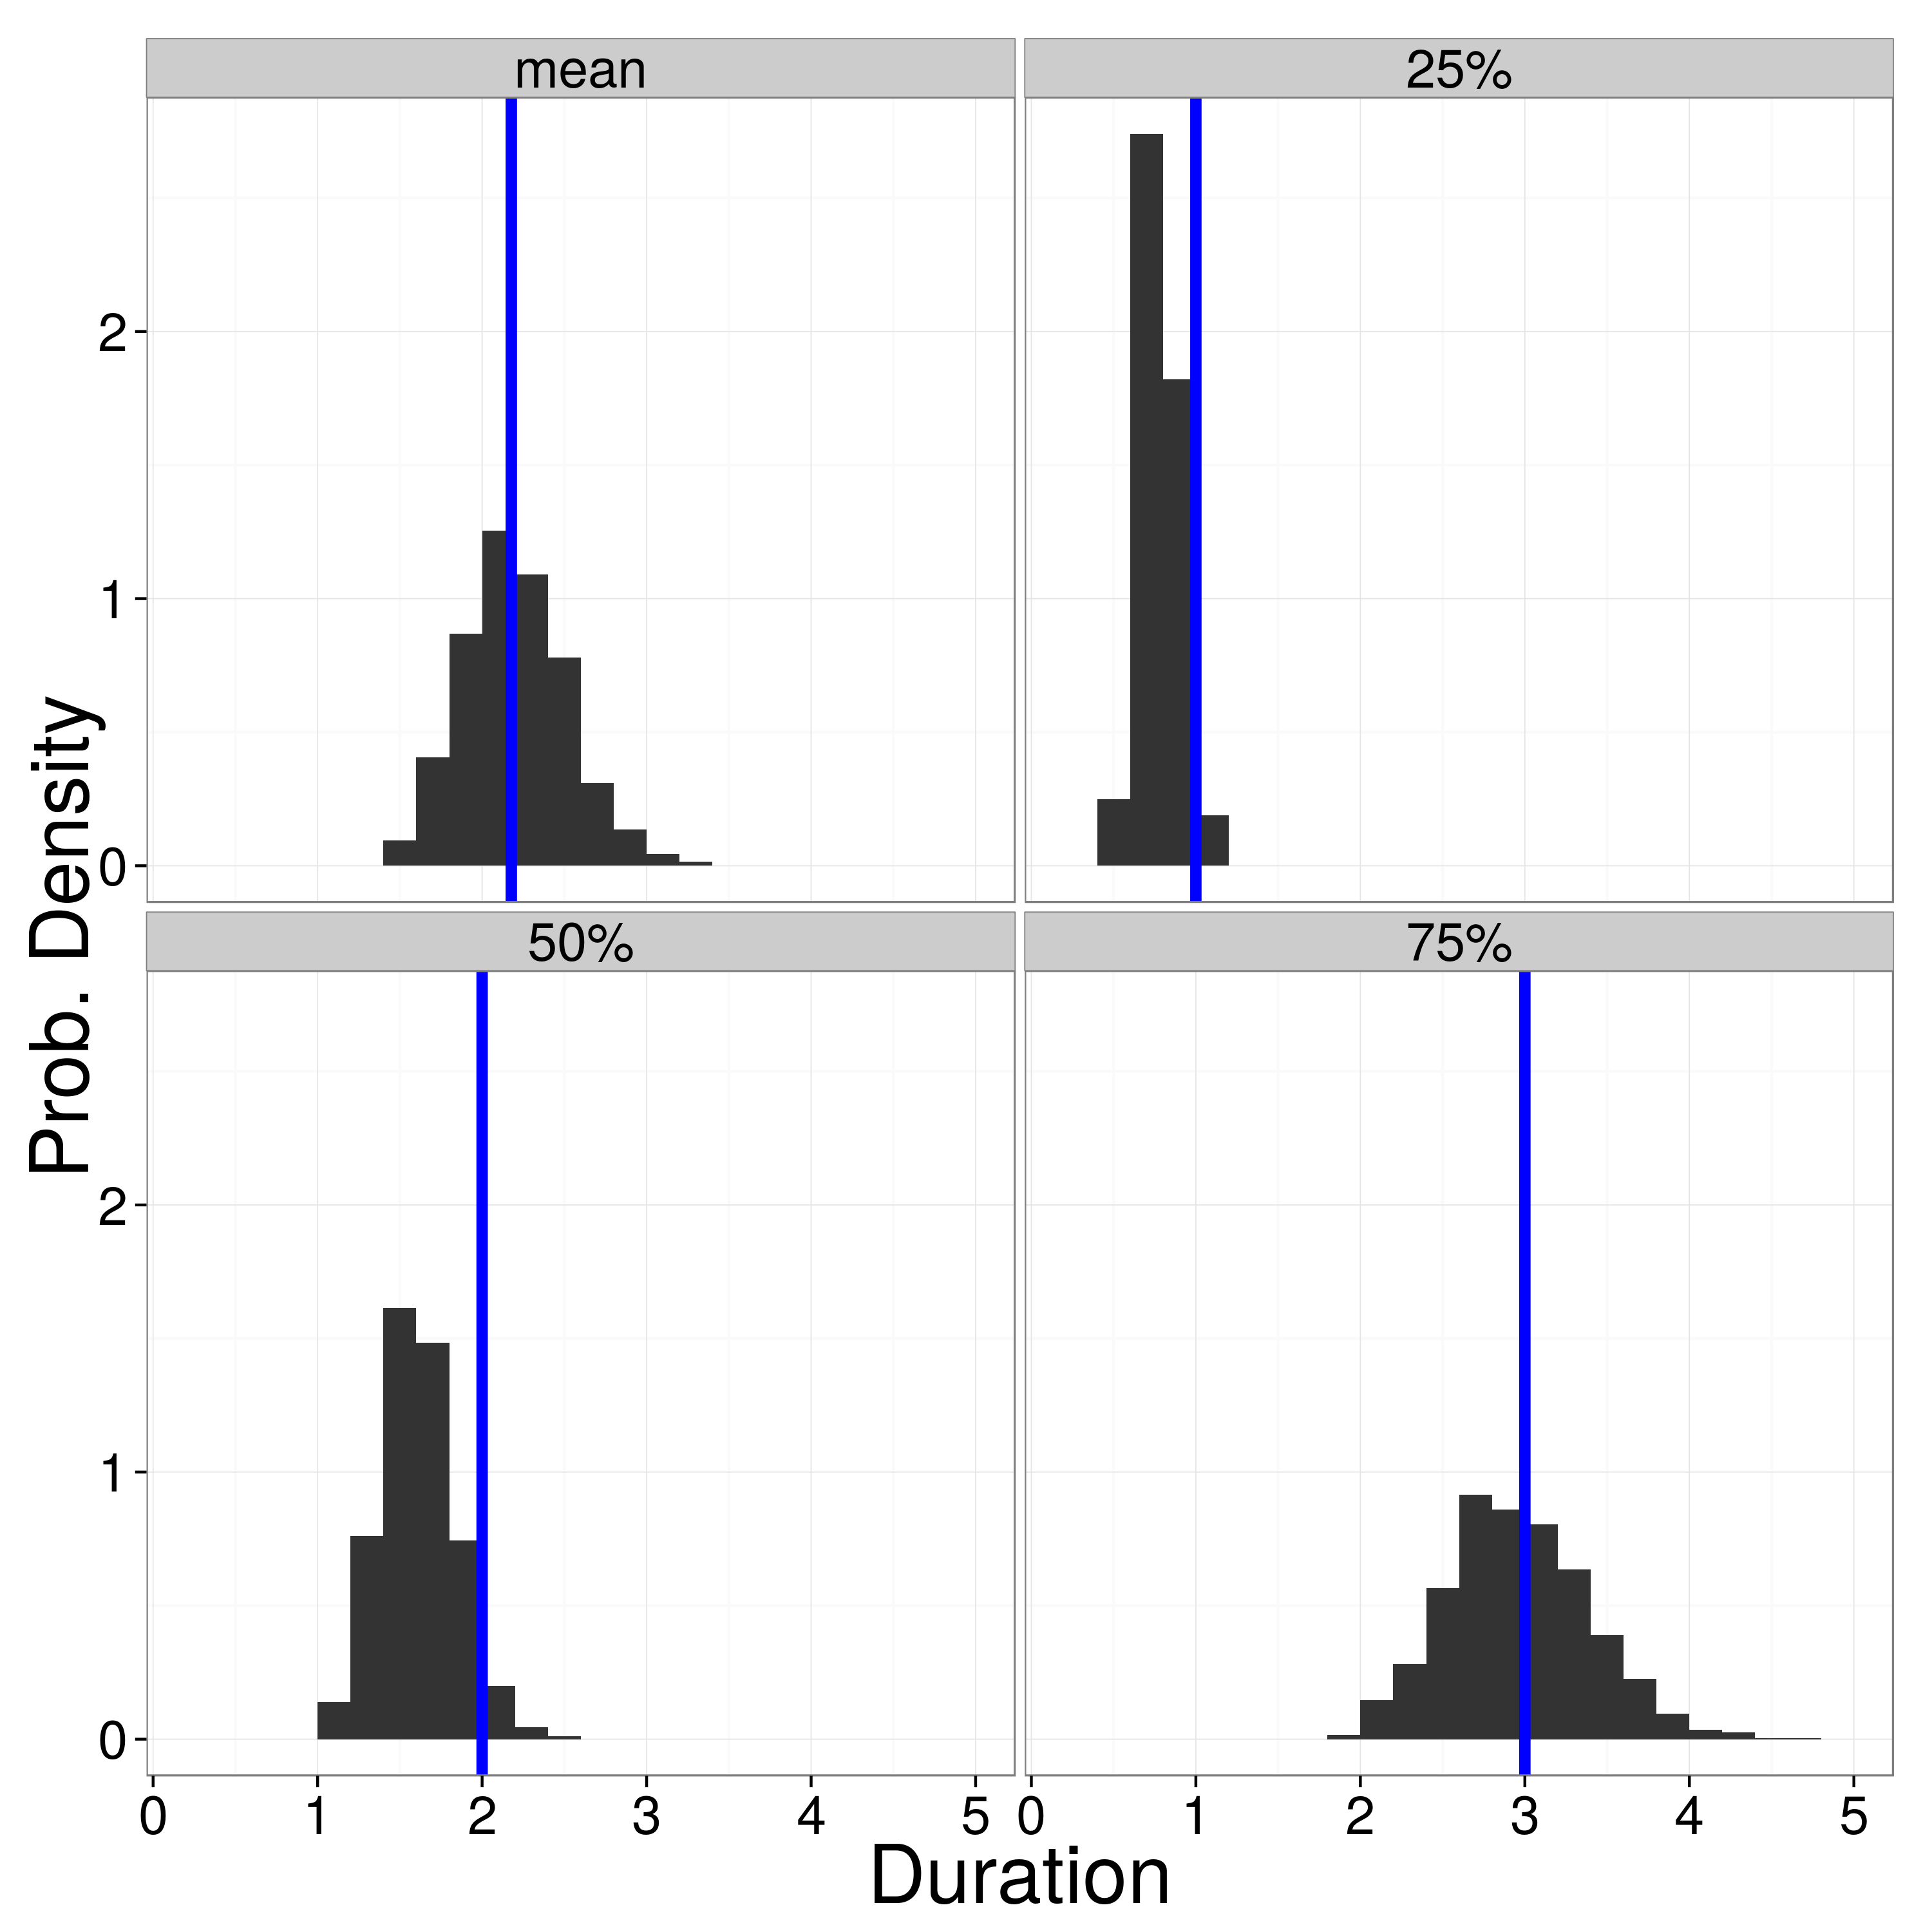
\includegraphics[height = 0.5\textheight, width = \textwidth, keepaspectratio = true]{figure/quant_ppc}
  \caption{The results of additional posterior predictive checks for four summaries of the observed durations, as labeled. Blue vertical indicate the observed value. None of the observed are significantly different from the posterior predictive distributions.}
  \label{fig:ppc_quant}
\end{figure}

\begin{figure}[ht]
  \centering
  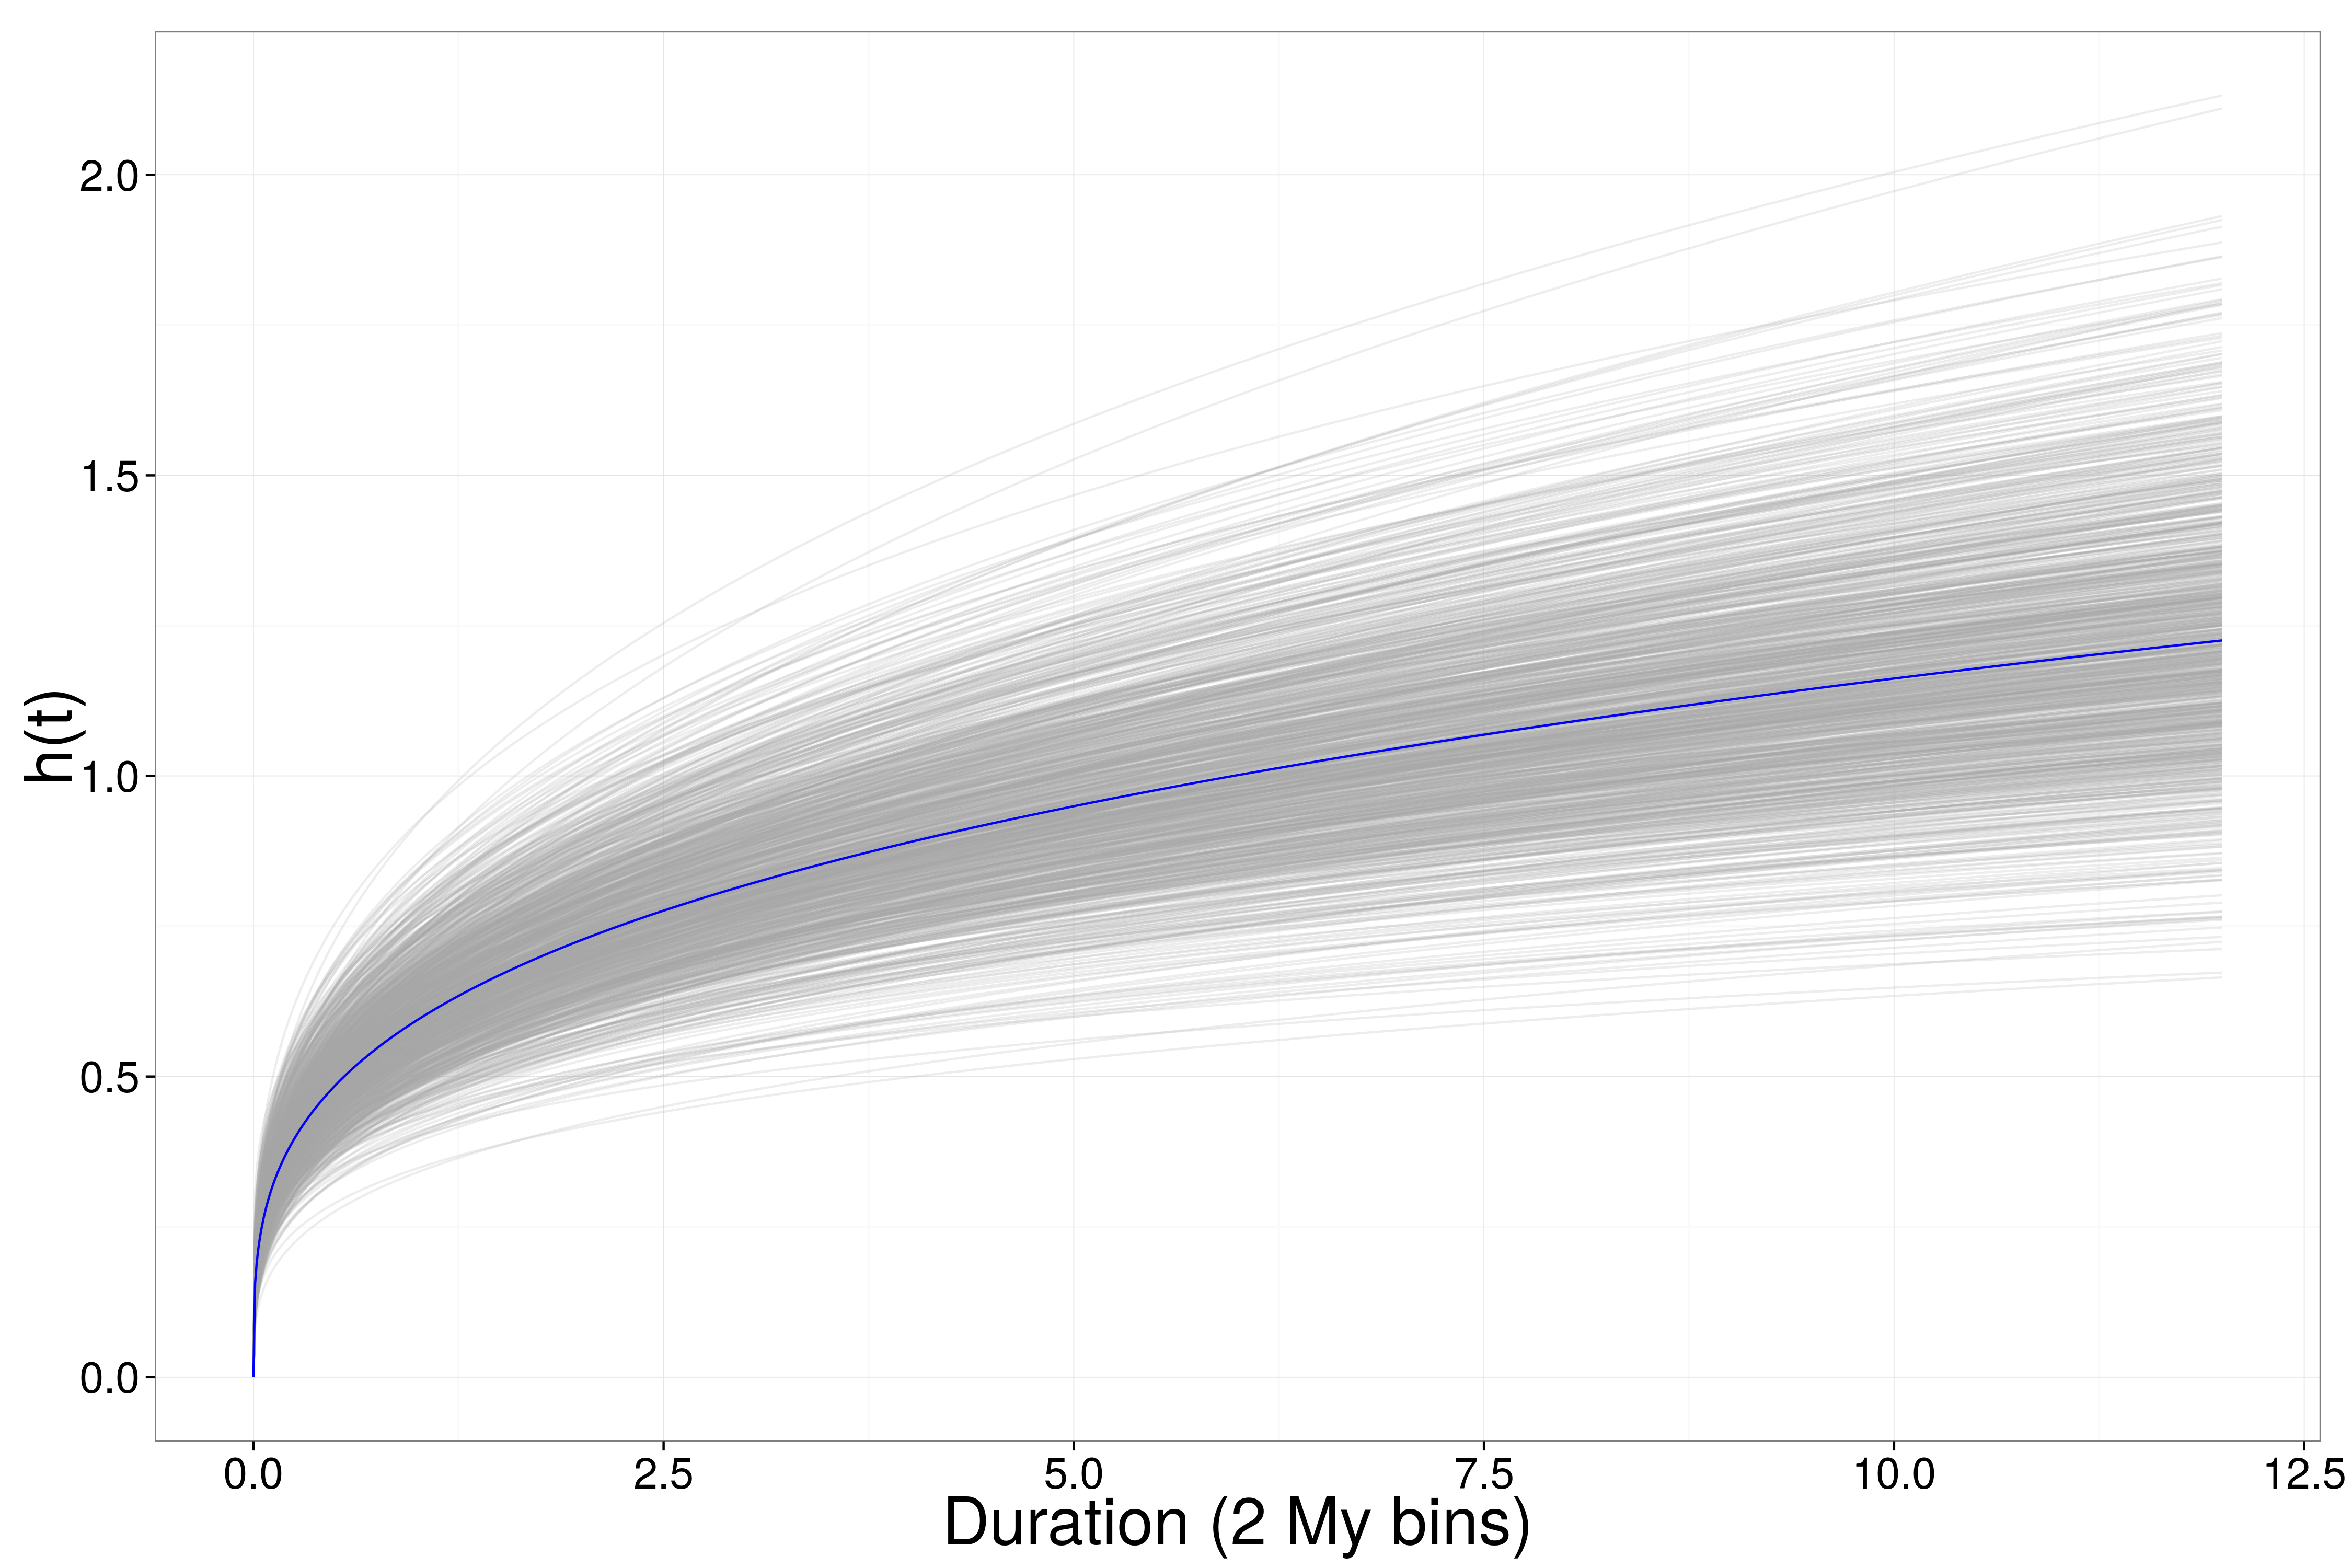
\includegraphics[height = 0.5\textheight, width = \textwidth, keepaspectratio = true]{figure/haz_est}
  \caption{100 estimates of the hazard function (\(h(t\)) for the observed species mean (grey), along with the median estimated hazard function. \(h(t)\) is an estimate of the rate at which a species of age \(t\) is expected to go extinct. Hazard functions were estimated from random draws from the estimated posterior distributions and evaluated with all covariate information set to 0, which corresponds to the expected duration of the mean species.}
  \label{fig:haz}
\end{figure}



\clearpage


\section{Supplementary tables}
% latex table generated in R 3.1.2 by xtable 1.7-4 package
% Thu Jan  8 17:45:30 2015
\begin{table}[c]
  \centering
  \begin{tabular}{rrrrrrrrr}
    & mean & sd & 2.5\% & 25\% & 50\% & 75\% & 97.5\% & \(\hat{R}\) \\ 
    \hline
    alpha & 1.29 & 0.03 & 1.23 & 1.27 & 1.29 & 1.31 & 1.36 & 1.00 \\ 
    intercept & -0.78 & 0.14 & -1.05 & -0.87 & -0.78 & -0.68 & -0.51 & 1.00 \\ 
    logit(occupancy) & -0.53 & 0.08 & -0.69 & -0.59 & -0.53 & -0.48 & -0.38 & 1.00 \\ 
    log(size) & -0.05 & 0.05 & -0.14 & -0.08 & -0.05 & -0.01 & 0.05 & 1.00 \\ 
    ground dwelling & -0.28 & 0.10 & -0.47 & -0.34 & -0.28 & -0.21 & -0.09 & 1.00 \\ 
    scansorial & -0.22 & 0.11 & -0.43 & -0.29 & -0.22 & -0.14 & -0.00 & 1.00 \\ 
    herbivore & 0.09 & 0.09 & -0.09 & 0.03 & 0.09 & 0.14 & 0.27 & 1.00 \\ 
    insectivore & 0.10 & 0.11 & -0.11 & 0.03 & 0.10 & 0.17 & 0.31 & 1.00 \\ 
    omnivore & -0.12 & 0.11 & -0.33 & -0.19 & -0.12 & -0.05 & 0.09 & 1.00 \\ 
    \hline
    sd cohort & 0.33 & 0.06 & 0.23 & 0.29 & 0.33 & 0.37 & 0.48 & 1.00 \\ 
    sd phylogeny & 0.11 & 0.05 & 0.03 & 0.07 & 0.10 & 0.14 & 0.23 & 1.03 \\ 
    \hline
  \end{tabular}
  \caption{Marginal posterior estimates for the praameters of interested based on 1000 posterior samples. The intercept can be interpreted as the estimate for the mean observed species. The other values are the effect of a trait on the expected species duration as expressed as deviation from the mean. The categorical variables are binary index variables where an observation is of that category or not. \(\hat{R}\) values of less than 1.1 indicate approximate chain convergence for the posterior samples.}
  \label{tab:post_sum}
\end{table}


\begin{table}[t!]
  \centering
  \caption{Species trait assignments in this study are a coarser version of the information available in the PBDB. Information was coarsened to improve per category sample size and uniformity and followed this table.}
  \begin{tabular}[ht]{ l | l | l }
    \hline
    \multicolumn{2}{ c |}{This study} & PBDB categories \\
    \hline \hline
    \multirow{4}{*}{Diet} & Carnivore & Carnivore \\
    & Herbivore & Browser, folivore, granivore, grazer, herbivore. \\
    & Insectivore & Insectivore. \\
    & Omnivore & Frugivore, omnivore. \\ 
    \hline
    \multirow{3}{*}{Locomotor} & Arboreal & Arboreal.\\
    & Ground dwelling & Fossorial, ground dwelling, semifossorial, saltatorial. \\
    & Scansorial & Scansorial. \\
    \hline
  \end{tabular}
  \label{tab:trait_cats}
\end{table}

\clearpage

\begin{table}[t!]
  \centering
  \begin{tabular}{l | l | l | l}
    Group & Equation & log(Measurement) & Source \\
    \hline
    General & \(\log(m) = 1.827x + 1.81\) & lower m1 area &  \cite{Legendre1986} \\
    General & \(\log(m) = 2.9677x - 5.6712\) & mandible length & \cite{Foster2009a} \\
    General & \(\log(m) = 3.68x - 3.83\) & skull length & \cite{Luo2001} \\
    Carnivores & \(\log(m) = 2.97x + 1.681\) & lower m1 length & \cite{VanValkenburgh1990} \\
    Insectivores & \(\log(m) = 1.628x + 1.726\) & lower m1 area & \cite{Bloch1998} \\
    Insectivores & \(\log(m) = 1.714x + 0.886\) & upper M1 area & \cite{Bloch1998} \\
    Lagomorph & \(\log(m) = 2.671x - 2.671\) & lower toothrow area & \cite{Tomiya2013} \\
    Lagomorph & \(\log(m) = 4.468x - 3.002\) & lower m1 length & \cite{Tomiya2013} \\
    Marsupials & \(\log(m) = 3.284x + 1.83\) & upper M1 length & \cite{Gordon2003} \\
    Marsupials & \(\log(m) = 1.733x + 1.571\) & upper M1 area & \cite{Gordon2003} \\
    Rodentia & \(\log(m) = 1.767x + 2.172\) & lower m1 area & \cite{Legendre1986} \\
    Ungulates & \(\log(m) = 1.516x + 3.757\) & lower m1 area & \cite{Mendoza2006} \\
    Ungulates & \(\log(m) = 3.076x + 2.366\) & lower m2 length & \cite{Mendoza2006} \\
    Ungulates & \(\log(m) = 1.518x + 2.792\) & lower m2 area & \cite{Mendoza2006} \\
    Ungulates & \(\log(m) = 3.113x - 1.374\) & lower toothrow length & \cite{Mendoza2006} \\
    \hline
  \end{tabular}
  \caption{CAPTION}
  \label{tab:mass_est}
\end{table}

\clearpage
\bibliography{newbib,packages}
\end{document}
